\chapter{Machine Learning}
\chaplabel{machineLearning}

\section{Purpose}
This is an introduction to pattern recognition/machine learning by creating a 
word recognition system on \href{https://edgeimpulse.com/}{Edge Impulse} and 
deploying it on the Nano RP2040 Connect. 

\section{Laboratory}
\subsection{Creating and Installing Voice Recognition}
\begin{enumerate}
  \item Go to the \href{https://edgeimpulse.com/}{Edge Impulse} website and create an 
account. 
  \item It is going to try to start you on a tutorial. These directions assume you quit 
      the tutorial.
  \item Find the blue ``+ Create new project'' button and press it 
  \item Enter a name for the project and press ``Create new project''
  \item Click on the Data acquisition tab on the left
  \item Upload a folder containing individual word samples one at a time
  \begin{enumerate}
    \item It can mess up if it tries to auto label the samples
    \item Label the samples according to what they represent (yes, no, noise, etc.)
    \item There is a zip file on Canvas named keywords2.zip which contains yes, no, noise, and unknown examples
    \item Follow the link in Resources to find a Google repository with more words if you want something else
    \item Making your own recordings can work, but will be time consuming since you need 5-10 min of examples 
            for each word you want recognized.
    \item Choose: Select folder, choose the folder, automatically split, Enter label so it should look 
            like Figure \ref{fig:edgeimpulseupload}.

  \begin{figure}[!htb]
    \centering
    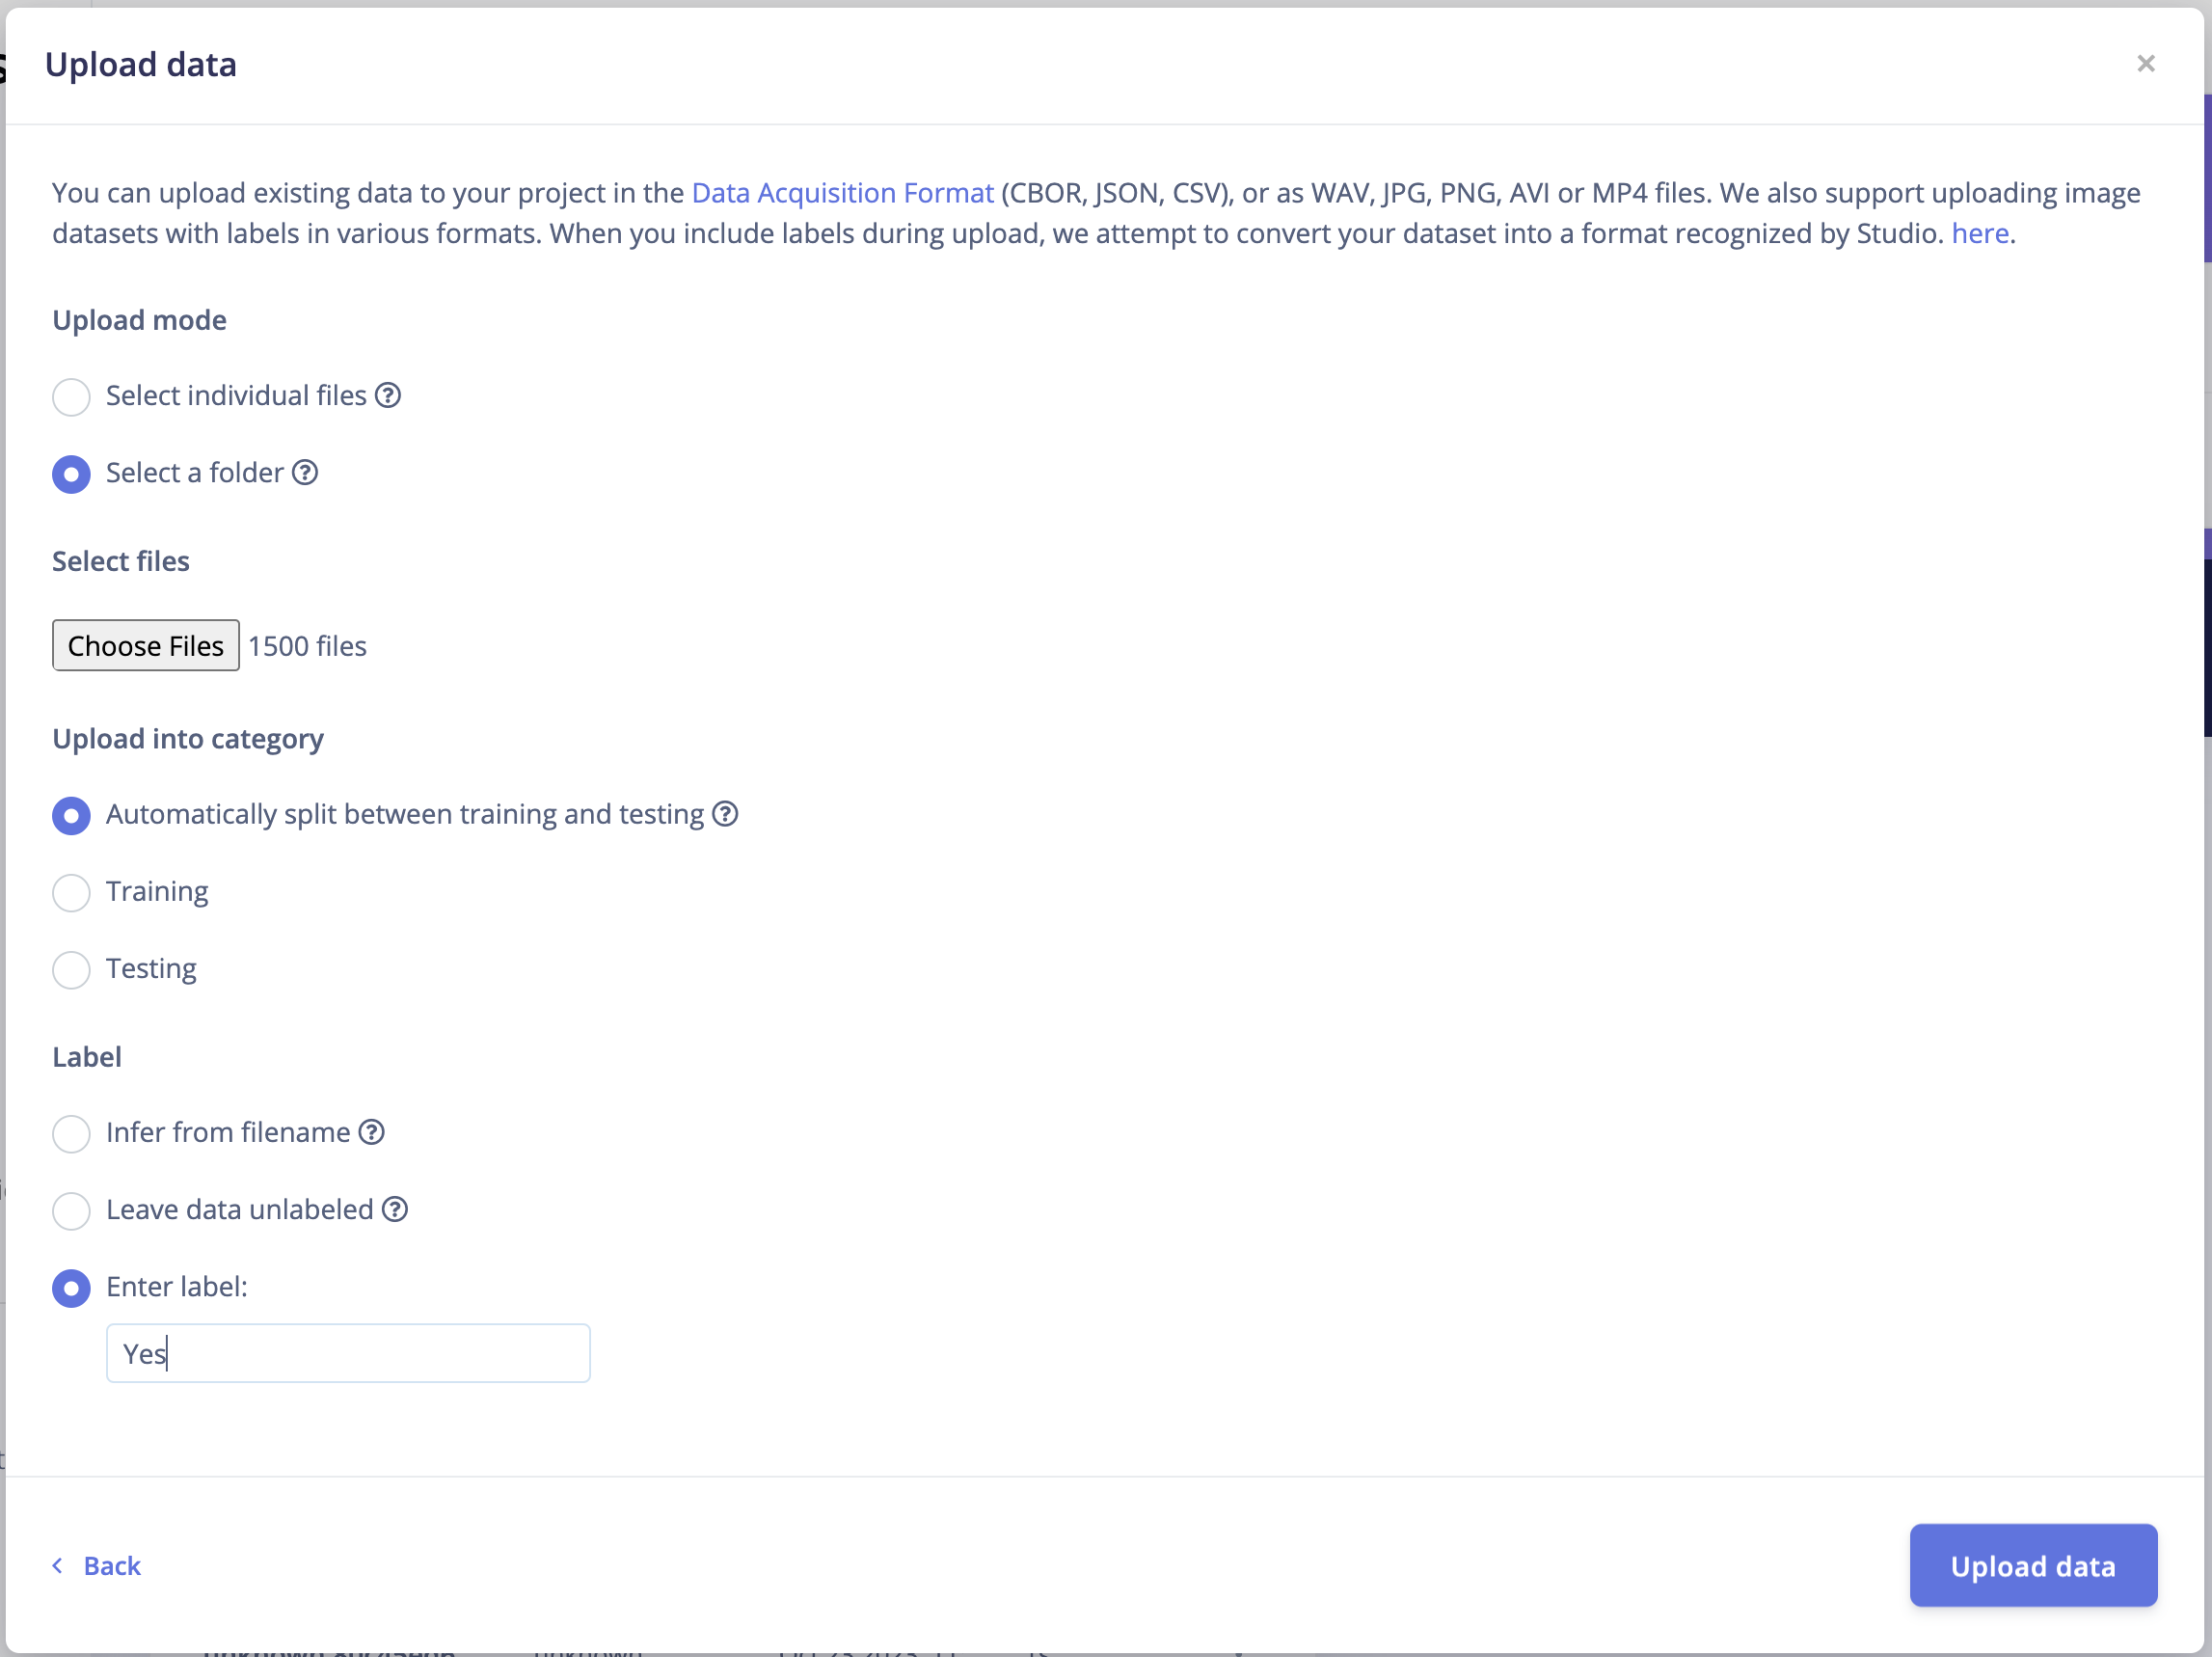
\includegraphics[scale=0.3]{machineLearning/upload.png}
    \caption{This shows a ready to upload set of files.}
    \label{fig:edgeimpulseupload}
  \end{figure} 

    \item Once your data is uploaded, the page should look similar to Figure~\ref{fig:edgeimpulsedata}
  \end{enumerate}

  \begin{figure}[!htb]
    \centering
    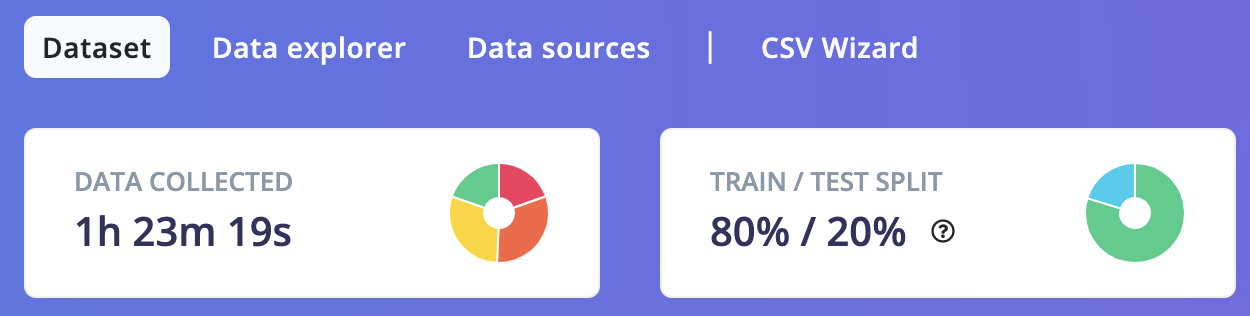
\includegraphics[scale=0.6]{machineLearning/data.png}
    \caption{Once the data is uploaded this figure shows what your project should look like.}
    \label{fig:edgeimpulsedata}
  \end{figure} 

  \item Click on Impulse design
  \item Leave it on Time series data, window of 1000 ms, window increase of 500 ms.
  \item Change the Frequency to 20000 Hz and leave Zero-pad checked
  \item Choose MFCC as the audio features
  \item Classification should have a small number of Output features 
          (4 in my example for no, noise, unknown, yes)
  \item The impulse should look like what is shown in Figure~\ref{fig:edgeimpulseimpulse}
  \item Click Save Impulse

  \begin{figure}[!htb]
    \centering
    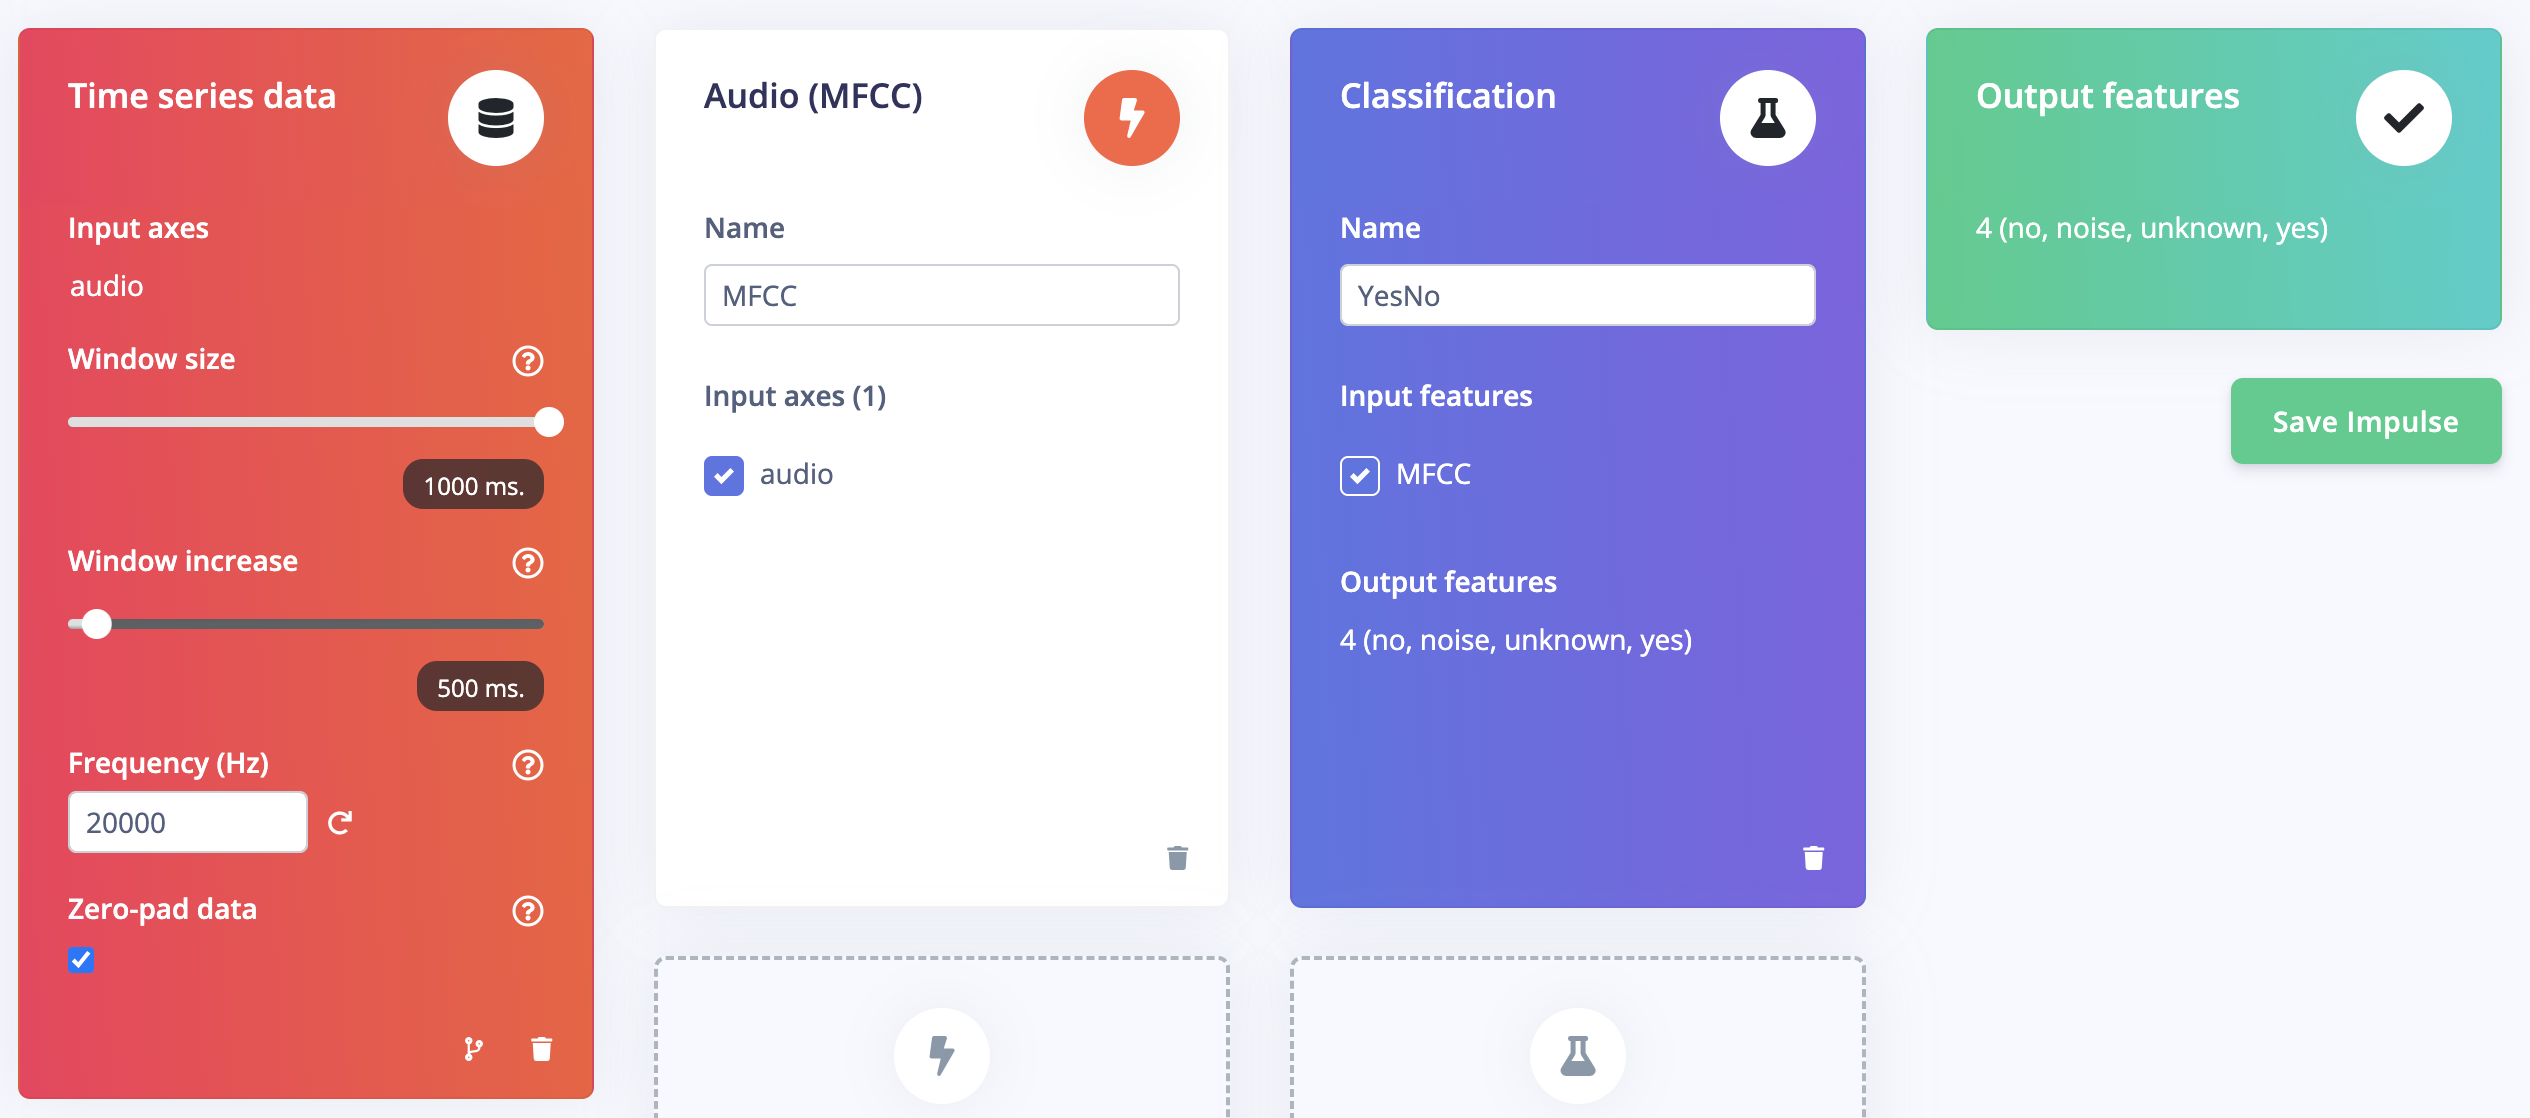
\includegraphics[scale=0.3]{machineLearning/Impulse.png}
    \caption{The impulse setup should look similar to this. Note the frequency is 20kHz.}
    \label{fig:edgeimpulseimpulse}
  \end{figure} 

  \item Click on MFCC
  \item Click on Save parameters
  \item Click on the Generate features tab
  \item Then click on the Generate features button. This will take awhile
  \item Once that finishes (green complete in console), click on your model 
          (name under MFCC)
  \item Change the number of training cycles to 50
  \item Change the Learning rate to 0.005
  \item Change the target (upper right) to Raspberry Pi RP2040 (Cortex-M0+ 133MHz)
  \item Click Start training. This will also take awhile. 
  \item After training, the page should look like Figure~\ref{fig:edgeimpulsetrained}

  \begin{figure}[!htb]
    \centering
    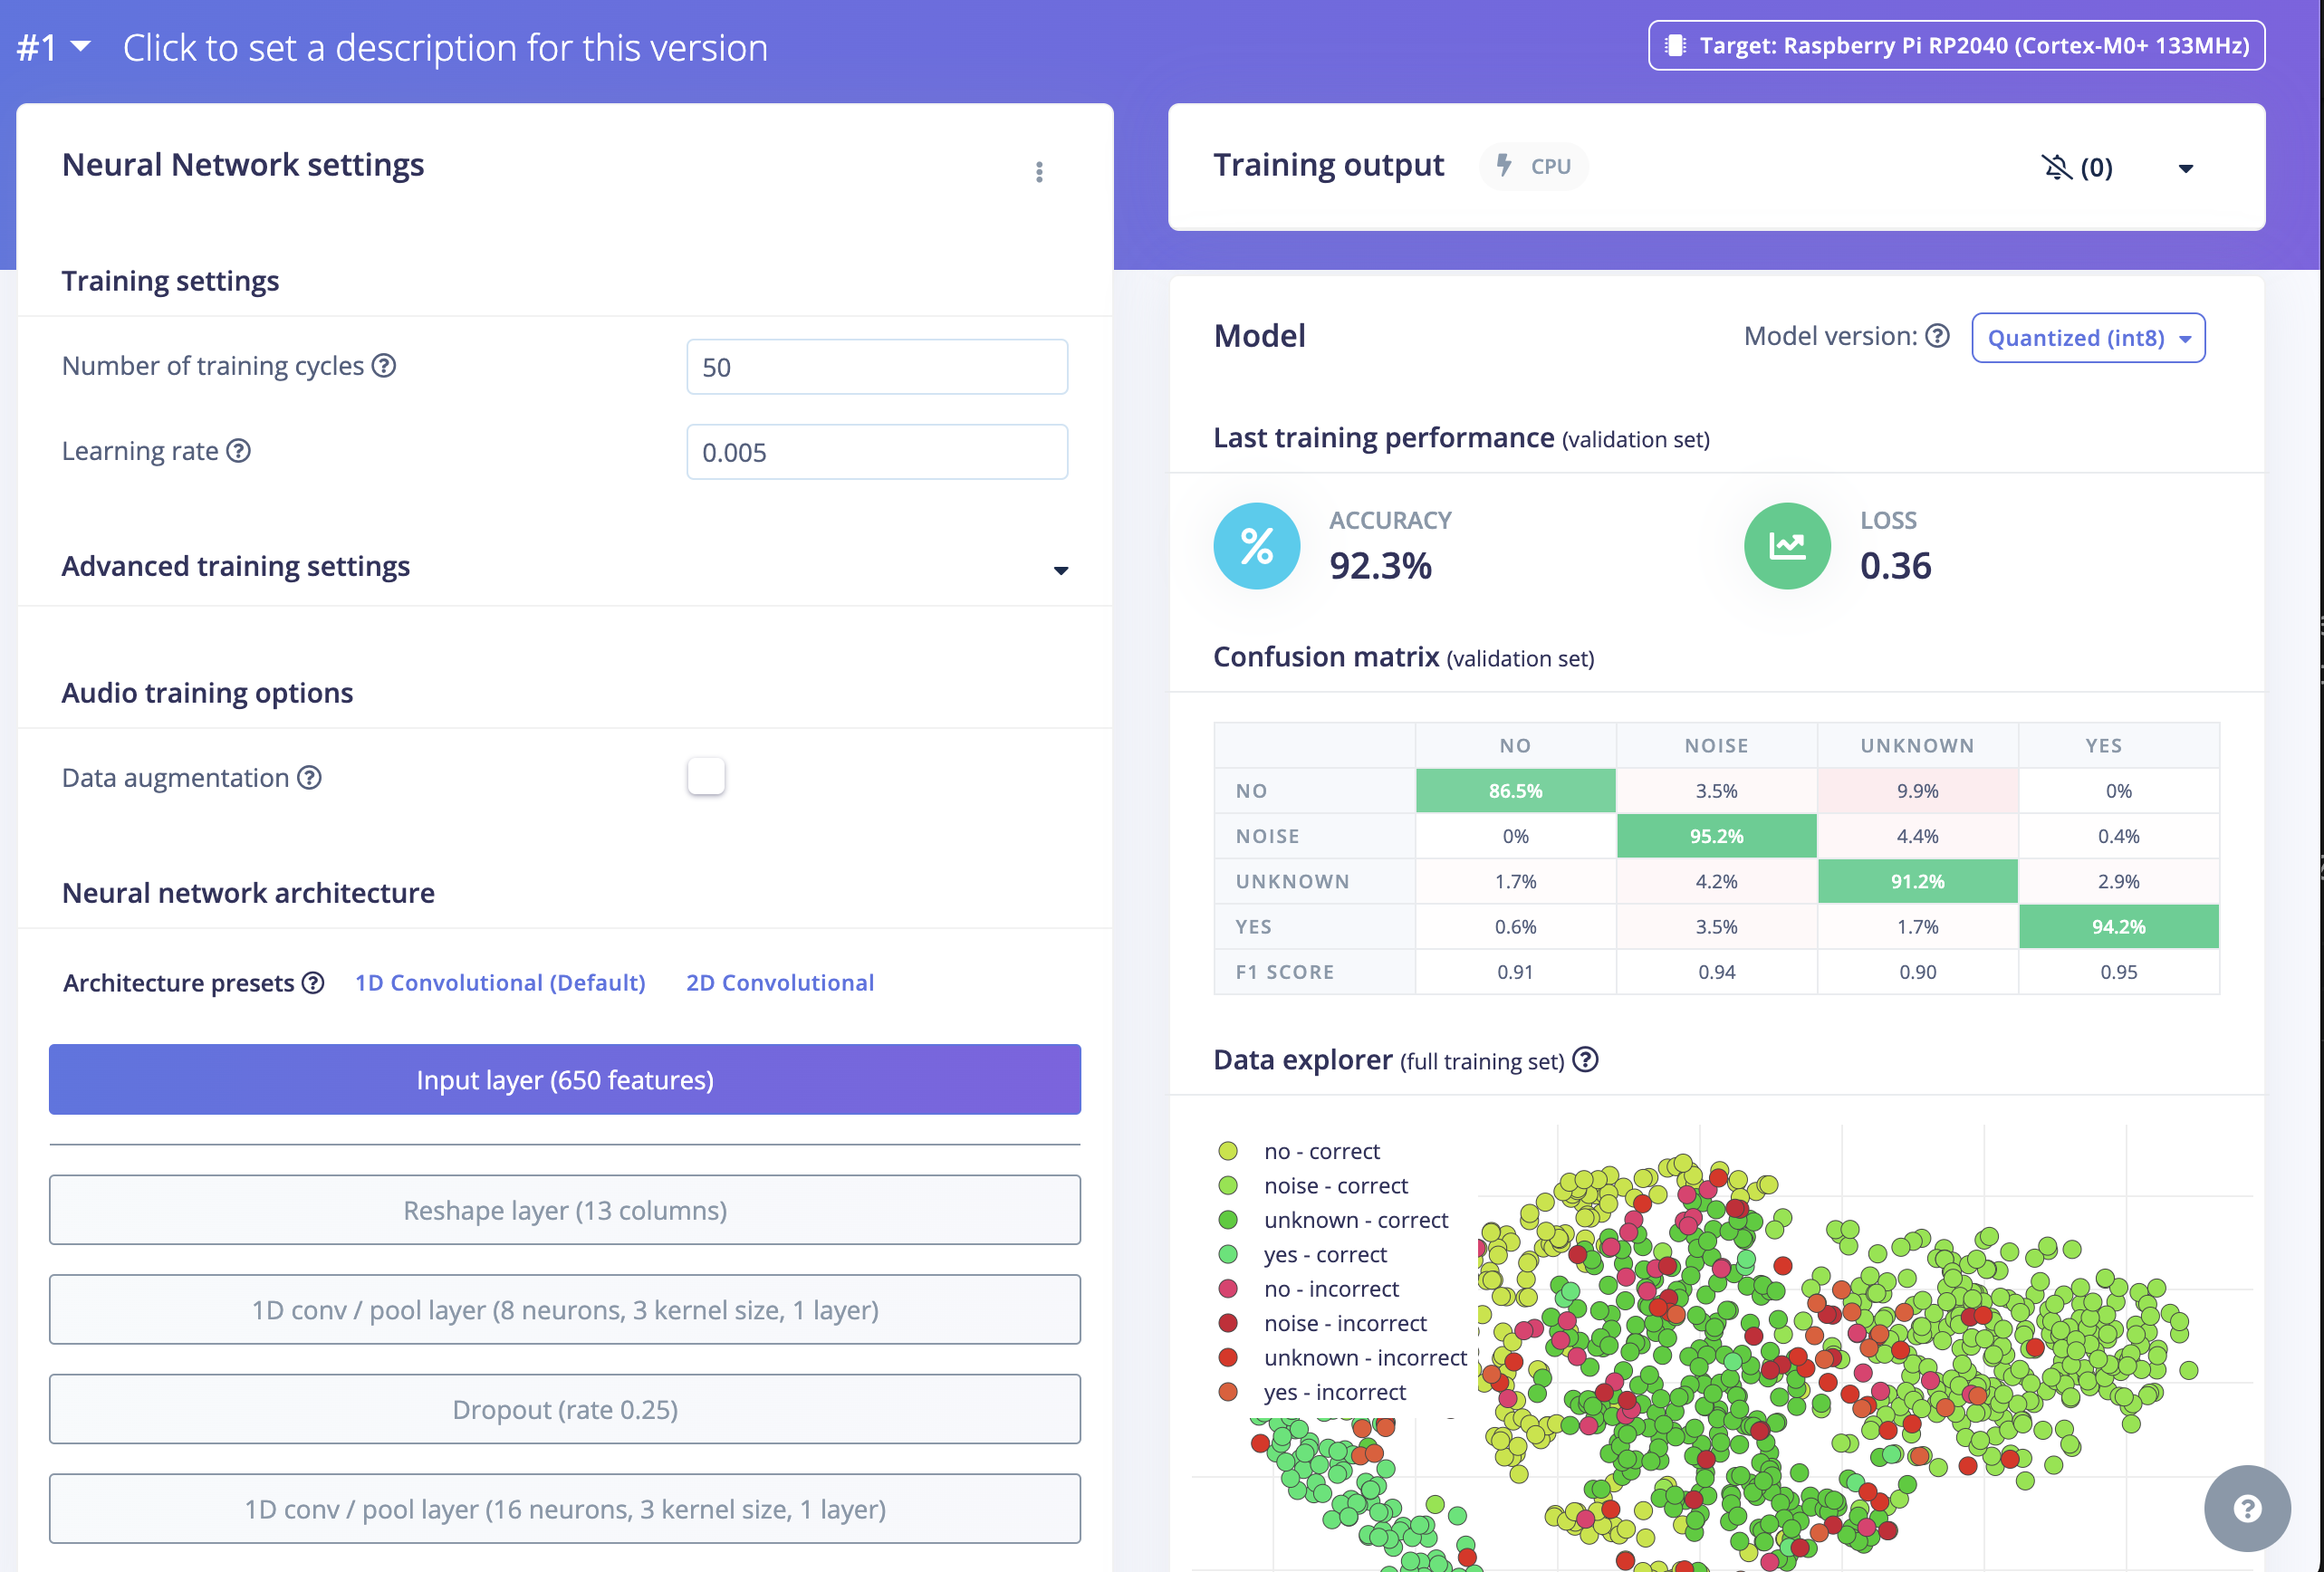
\includegraphics[scale=0.3]{machineLearning/trained.png}
    \caption{The fully trained model should result in something like this. Note the Target.}
    \label{fig:edgeimpulsetrained}
  \end{figure} 

  \item Once that completes, click on Deployment on the left 
  \item Search deployment options for Arduino library so that it looks like Figure \ref{fig:edgeimpulsearduino}

  \begin{figure}[!htb]
    \centering
    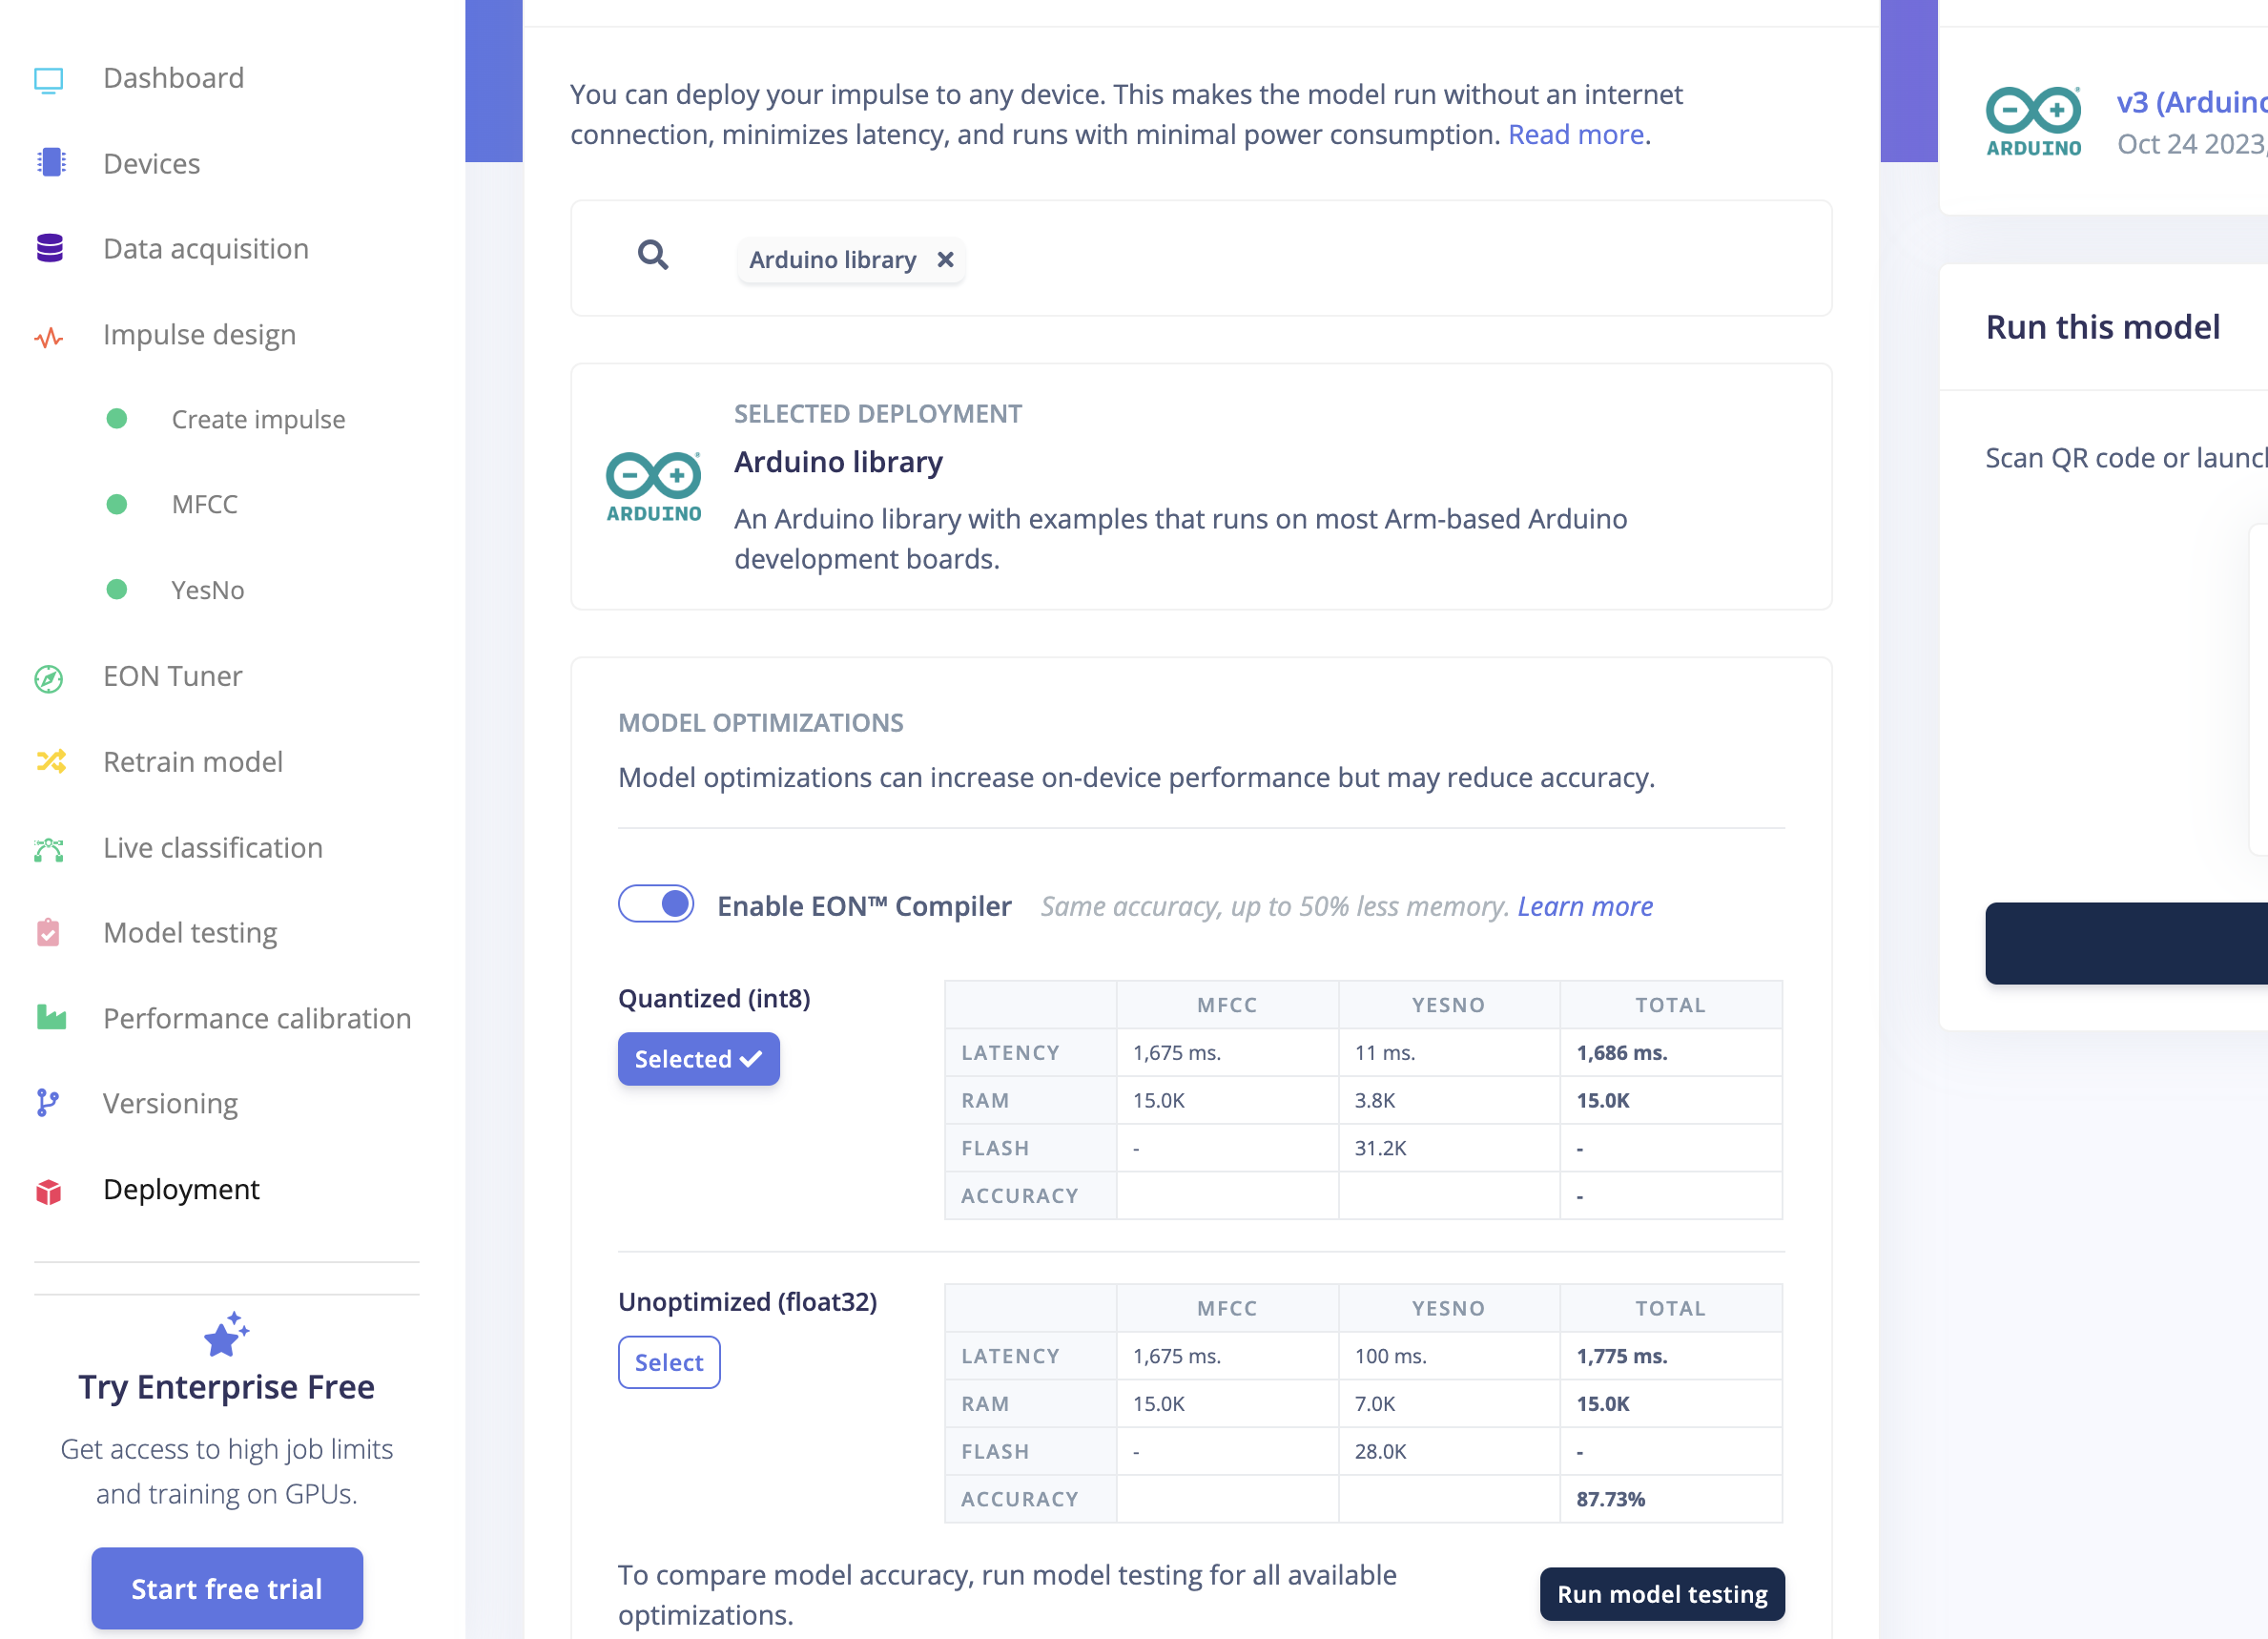
\includegraphics[scale=0.3]{machineLearning/arduino.png}
    \caption{This shows a model read to build as an Arduino library.}
    \label{fig:edgeimpulsearduino}
  \end{figure} 

  \item Click Build
  \item After it finishes it should download a zip file and show some directions
  \item Follow the directions to install the library and open the RP2040 Microphone example 
  \item Try running the example and see if the Serial output shows the word you say as the 
          most likely thing heard. Note that it only listens every few seconds. Watch the 
          serial port output for when it's recording.
\end{enumerate}

\subsection{Adding Improvements}
The library example as written does not output which class is the most likely candidate.

\begin{enumerate}
  \item Improve the \lstinline|print_inference_result| function to print out the name 
          of the most likely class and its probability.
  \item Have the script play a different tone for recognition of the classes of interest 
          (yes, no in my example)
\end{enumerate}

You should also be able to make it drive quite easily as a reaction to your spoken word. To make 
the NeoPixels work, use the \lstinline|NeoPixelConnect| library. Initialize it to use PIO 1, 
state machine 0 like this before your \lstinline|setup()| function:
\begin{lstlisting}
  #define NEO_PIN   17
  #define NEO_COUNT 17
  NeoPixelConnect strip(NEO_PIN, NEO_COUNT, pio1, 0);
\end{lstlisting}

In your subsequent functions, the NeoPixels are controlled as shown:
\begin{lstlisting}
  // sets LED 6 to (R,G,B) of (100,0,0) and 
  // immediately displays it
  strip.neoPixelSetValue(6,100,0,0,true);
\end{lstlisting}

I suspect the screen will not work, but have not tried it yet.

\section{Extras}
If you'd like to see some examples of already created recognition models, try out the 
capabilities of the IMU on your board. 

\subsection{Download Examples}
There is a zip file on Canvas named LSM6DSOX\_Examples.zip. Download and extract the zip 
file. Move the resulting folder into your sketch directory (usually named arduino or Arduino 
inside your Documents folder). Now try opening one of the examples from within the Arduino IDE.
If you can find it in your File $\rightarrow$ Sketchbook menu, you have put them in the right
place.

\subsection{Install Library}
Install the STM32duino\_LSM6DSOX library in the Arduino IDE since these examples rely on 
it for the interface to the IMU.

\subsection{Running Examples}
Run each of the following examples noting that the outputs will all be via the serial port:

\subsubsection{6D Orientation}
Open the example named LSM6DSOX\_6DOrientation. Compile and upload it to the board. When it
runs, it should output a drawing indicating the orientation as you rotate the board.

\subsubsection{Free Fall Detection}
Don't drop or throw the board! Open the example named LSM6DSOX\_FreeFallDetection. Compile 
and upload it to your board. When it is running, raise and lower the board while holding it 
and it should send an output when it thinks it is in free fall. 

\subsubsection{Pedometer}
Open the example named LSM6DSOX\_Pedometer. Compile and upload it to the board. Once it is 
running it should print out the number of steps periodically. Shake the board up and down 
to imitate walking and it should increment the counter.

\subsubsection{Tap Detection}
Open the example named LSM6DSOX\_TapDetect. Compile and upload it to the board. Once it is 
running try tapping the side of the board/module (not front, back, or top). The serial should 
output single tap and double tap as it thinks it is tapped.

\subsubsection{Tilt Detection}
Open the example named LSM6DSOX\_TiltDetection. Compile and upload it to the board. Once it is 
running try tilting the board after letting it sit in one orientation for a bit. It should 
trigger a serial output when you move the board.

\subsubsection{Wake Up Detection}
Open the example named LSM6DSOX\_WakeUpDetection. Compile and upload it to the board. Once it is 
running try moving the board after letting it sit still for a bit. It should trigger a serial 
output when you move the board.

\subsubsection{Machine Learning Example}
Open the example named LSM6DSOX\_MLC. Compile and upload it to the board. Once it is 
running try moving the board to simulate walking, running, biking, driving, unknown, and 
staying stationary. Walking and jogging are the easiest to get with vertical motion (Z-axis). 
Biking seems to be lateral motion (X- or Y-axis). I have seen driving once but don't remember 
how I got it. I have never seen unknown.

% \subsection{Using the Examples}
% Take one or more of the examples and do something with them. It could be as simple as 
% adding sound or screen output to the example(s) or something more.


\section{Turn In}
Turn in the following:
\begin{enumerate}
    \item Have either the TA or the instructor sign-off on your lab
    \item A PDF of your sketch.
    \item .ino versions of your sketch.
    \item Fill out the end of lab quiz prior to leaving. Note that it includes asking you 
            for the output of the \lstinline$getIDs$ sketch. 
\end{enumerate}

\section{Resources}\label{sec:machinelearningresources}
\begin{enumerate}
    \item \href{https://pietropoluzzi.it/blog/ml/edge-impulse/voice-recognition/}{Voice recognition tutorial}
    \item \href{https://docs.edgeimpulse.com/docs/pre-built-datasets/keyword-spotting}{Yes, no, unkown, noise dataset}
    \item \href{https://blog.research.google/2017/08/launching-speech-commands-dataset.html}{Google keywords dataset}
    \item \href{https://github.com/stm32duino/LSM6DSOX/blob/main/src/LSM6DSOXSensor.h}{LSM6DSOX Library Header}
    \item \href{https://www.st.com/resource/en/datasheet/lsm6dsox.pdf}{LSM6DSOX Datasheet}
    \item PCB Schematic and Layout - see 
            \href{https://github.com/semcneil/Fundamentals-of-Microcontrollers-Manual}{class manual} 
            in the Arduino Startup $\rightarrow$ Schematics and PCB section
\end{enumerate}

